\let\negmedspace\undefined
\let\negthickspace\undefined
\documentclass[journal]{IEEEtran}
\usepackage[a5paper, margin=10mm, onecolumn]{geometry}
%\usepackage{lmodern} % Ensure lmodern is loaded for pdflatex
\usepackage{tfrupee} % Include tfrupee package

\setlength{\headheight}{1cm} % Set the height of the header box
\setlength{\headsep}{0mm}     % Set the distance between the header box and the top of the text

\usepackage{gvv-book}
\usepackage{gvv}
\usepackage{cite}
\usepackage{amsmath,amssymb,amsfonts,amsthm}
\usepackage{algorithmic}
\usepackage{graphicx}
\usepackage{textcomp}
\usepackage{xcolor}
\usepackage{txfonts}
\usepackage{listings}
\usepackage{enumitem}
\usepackage{mathtools}
\usepackage{gensymb}
\usepackage{comment}
\usepackage[breaklinks=true]{hyperref}
\usepackage{tkz-euclide} 
\usepackage{listings}
% \usepackage{gvv}                                        
\def\inputGnumericTable{}                                 
\usepackage[latin1]{inputenc}                                
\usepackage{color}                                            
\usepackage{array}                                            
\usepackage{longtable}                                       
\usepackage{calc}                                             
\usepackage{multirow}                                         
\usepackage{hhline}                                           
\usepackage{ifthen}                                           
\usepackage{lscape}
\begin{document}

\bibliographystyle{IEEEtran}
\vspace{3cm}

\title{1.5.21}
\author{EE25BTECH11033 - Kavin}
% \maketitle
% \newpage
% \bigskip
{\let\newpage\relax\maketitle}

\renewcommand{\thefigure}{\theenumi}
\renewcommand{\thetable}{\theenumi}
\setlength{\intextsep}{10pt} % Space between text and floats
\textbf{Question}:\\
Find the ratio in which $\vec{P}(4,m)$ divides the line segment joining the points $\vec{A}(2,3)$ and $\vec{B}(6,-3)$. Hence, find $m$.\\
\bigskip


\textbf{Solution}:\\
Let the vector $\vec{P}$ be 
\begin{align}
    \vec{P}=\begin{myvec}{4\\m}\end{myvec} \;, 
\end{align}
Given the points,
\begin{align}
    \vec{A}=\begin{myvec}{2\\3}\end{myvec}
    \vec{B}=\begin{myvec}{6\\-3}\end{myvec}
\end{align}
\bigskip
The points \vec{A}, \vec{P}, \vec{B} are collinear.\\
Points $\vec{A}, \vec{P}, \vec{B}$ are defined to be collinear if 
		\begin{align}
			\label{eq:line-rank-2}
			\rank{\myvec{\vec{P}-\vec{A}& \vec{B}-\vec{A}}} = 1\\
            \vec{P}-\vec{A} = \myvec{2\\m-3}\\
            \vec{B}-\vec{A} = \myvec{4\\-6}\\
            \myvec{\vec{P}-\vec{A}& \vec{B}-\vec{A}} = \myvec{2 & 4\\m-3 & -6}
		\end{align}
\begin{center}
$R_2 \rightarrow 2R_2 + 3R_1 \implies \myvec{2 & 4\\2m & 0}$
\end{center}
For rank $1$, the second row must be zero:
\begin{align}
    2m=0 \implies m=0
\end{align}
\begin{center}
$\therefore \vec{P}=\begin{myvec}{4\\0}\end{myvec}$
\end{center}
\\
Section formula for a vector $\vec{P}$ which divides the line formed by vectors $\vec{A}$ and $\vec{B}$ in the ratio k:1 is given by
\begin{align}
    \vec{P}=\frac{k\vec{B}+\vec{A}}{k+1}
\end{align}
\begin{align}
			k\brak{\vec{P}-\vec{B}}&= \vec{A}-\vec{P}
\end{align}
\begin{align}
    \implies k &=
			\frac{\brak{\vec{A}-\vec{P}}^{\top}\brak{\vec{P}-\vec{B}}}{\norm{\vec{P}-\vec{B}}^2}
			\label{eq:section_formula-k}
\end{align}
\bigskip
\begin{align}
\brak{\vec{A}-\vec{P}}^{\top}\brak{\vec{P}-\vec{B}} = \myvec{-2 & 3}\myvec{-2\\3} = 13\\
{\norm{\vec{P}-\vec{B}}^2} = \brak{\sqrt{2^2 + 3^2}}^2 = 13
\end{align}

\begin{align}
\implies k &= 1
\end{align}

Therefore the ratio in which $\vec{P}$ divides the line segment joining the points $\vec{A}$ and $\vec{B}$ is $1:1$\\
\\
See Fig. 0 ,
\begin{figure}[H]
\begin{center}
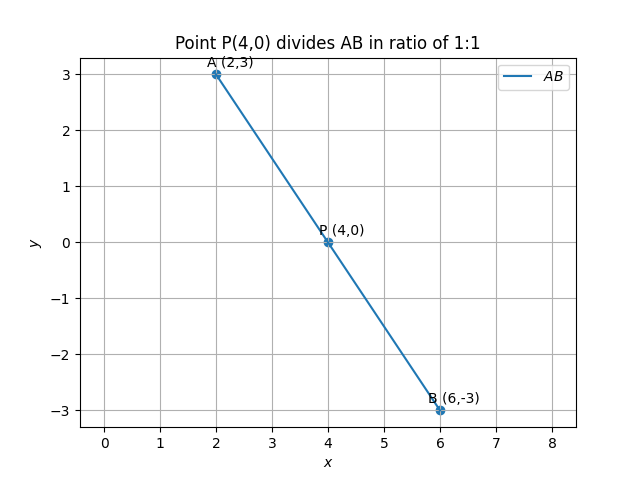
\includegraphics[width=0.6\columnwidth]{figs/fig.png}
\end{center}
\caption{}
\label{fig:Fig1}
\end{figure}



\end{document}

